%*****************************************
\chapter{Introduction}
\label{ch:introduction}
%*****************************************
\hint{This chapter should motivate the thesis, provide a clear description of the problem to be solved, and describe the major contributions of this thesis.}

\section{Motivation}
What is the motivation for doing research in this area?

\section{Problem Statement and Contribution}
What is the problem that should be solved with this thesis with its related research question?
What are the scientific contributions of your thesis to the field?

\section{Outline}
How is the rest of this thesis structured?



%*****************************************
\chapter{Background}
\label{ch:background}
%*****************************************
\hint{This chapter should give a comprehensive overview on the background necessary to understand the thesis.}


\section{Background Topic 1}
\section{Background Topic 2}
\section{Summary}


%*****************************************
\chapter{Related Work}
\label{ch:relatedwork}
%*****************************************
\hint{This chapter should give a comprehensive overview on the related work done by other authors followed by an analysis why the existing related work is not capable of solving the problem described in the introduction.}
\section{Related Work Area 1}

\begin{figure}[htb]
	\centering
 	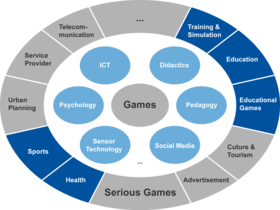
\includegraphics[width=0.5\textwidth]{gfx/sg-circle.png}  	  	 	
	\caption{Serious Games circle.}
	\label{fig:example1}
\end{figure}

\section{Related Work Area 2}

\begin{figure}[htb]
	\centering	
	\subcaptionbox{Alternative Serious Games Circle 1 %
		\label{fig:example_2}}%
 		[.48\linewidth]{
  		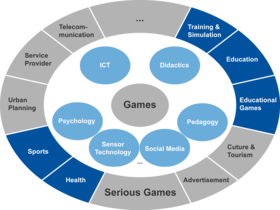
\includegraphics[width=0.35\textwidth]{gfx/sg-smiley.png} 	
  	}  	
  	~
  	\subcaptionbox{Alternative Serious Games Circle 2 %
  		\label{fig:example_3}}
 		[.48\linewidth]{
  		
\includegraphics[width=0.35\textwidth]{gfx/sg-circle_improved.png}  	
  	}	  
  		
	\caption{Alternatives of Serious Games circle.}
	\label{fig:ex_2_3}
\end{figure}

\section{Analysis of Related Work}

\section{Summary}

%*****************************************
\chapter{Design}
\label{ch:design}
%*****************************************
\hint{This chapter should describe the design of the own approach on a conceptional level without mentioning the implementation details.}

\section{Requirements and Assumptions}

\section{System Overview}

\subsection{Component 1}

\subsection{Component 2}

\section{Summary}

%*****************************************
\chapter{Implementation}
\label{ch:implementation}
%*****************************************

\hint{This chapter should describe the details of the implementation addressing the following questions: \\ \\
1. What are the design decisions made? \\
2. What is the environment the approach is developed in? \\
3. How are components mapped to classes of the source code? \\
4. How do the components interact with each other?  \\
5. What are limitations of the implementation? }
\section{Design Decisions}

\section{Architecture}

\section{Interaction of Components}

\section{Summary}

%*****************************************
\chapter{Evaluation}
\label{ch:evaluation}
%*****************************************
\hint{This chapter should describe how the evaluation of the implemented mechanism was done. \\ \\
1. Which evaluation method is used and why? Simulations, prototype? \\
2. What is the goal of the evaluation? Comparison? Proof of concept? \\
3. Wich metrics are used for characterizing the performance, costs, fairness, and efficiency of the system?\\
4. What are the parameter settings used in the evaluation and why? If possible always justify why a certain threshold has been chose for a particular parameter.  \\
5. What is the outcome of the evaluation? }
\section{Goal and Methodology}

\section{Evaluation Setup}

\begin{table}[htb]
\centering
	\begin{tabular}{ll}
	    \toprule
		\textbf{Parameter} & \textbf{Value} \\
		\midrule
		P1.1 & V1.1 \\
		P1.2 & V1.2 \\
		P1.3 & V1.3 \\
		\midrule
		P2 & V3 \\
		\midrule		
		P3 & V4 \\
		\bottomrule
	\end{tabular}
	
	\caption{Evaluation Parameters}
	\label{tab:eval_params}
\end{table}

\section{Evaluation Results}

\section{Analysis of Results}


%*****************************************
\chapter{Conclusions}
\label{ch:closure}
%*****************************************

\hint{This chapter should self-critically summarize the thesis and describe the main contributions of the thesis. Subsequently, it should describe possible future work in the context of the thesis. What are limitations of the developed solutions? Which things can be improved?}

\section{Summary}

\section{Contributions}

\section{Future Work}

\section{Final Remarks}
